\documentclass[12pt]{article}

% set margins and spacing
\addtolength{\textwidth}{1.3in}
\addtolength{\oddsidemargin}{-.65in} %left margin
\addtolength{\evensidemargin}{-.65in}
\setlength{\textheight}{9in}
\setlength{\topmargin}{-.5in}
\setlength{\headheight}{0.0in}
\setlength{\footskip}{.375in}
\renewcommand{\baselinestretch}{1.0}
\linespread{1.3}

% load miscellaneous packages
\usepackage{csquotes}
\usepackage[american]{babel}
\usepackage[usenames,dvipsnames]{color}
\usepackage{graphicx,amsbsy,amssymb, amsmath, amsthm, MnSymbol,bbding,times, verbatim,bm,pifont,pdfsync,setspace,natbib}

% enable hyperlinks and table of contents
\usepackage[pdftex,
bookmarks=true,
bookmarksnumbered=false,
pdfview=fitH,
bookmarksopen=true,hyperfootnotes=false]{hyperref}

% define environments
\newtheorem{definition}{Definition}
\newtheorem{fact}{Fact}
\newtheorem{result}{Result}
\newtheorem{proposition}{Proposition}



\begin{document}
\title{The Effect of Establishment Size on Work Place Accidents}
\author{Anna\thanks{Email: asrupert@syr.edu} \and Tomoyoshi\thanks{Email: ttakita@syr.edu} \and Yuhan\thanks{Email: ywang399@syr.edu}\and Will\thanks{Email: wmwaghor@syr.edu}}
\date{\vskip-.1in \today }
\maketitle

\vskip.3in
\begin{center} {\bf Abstract} \end{center}

\begin{quote}
This research investigates the impact of establishment size on workplace safety, specifically examining the correlation between establishment size and the rate of injuries. Motivated by the role of workplace safety in employee well-being and business success, our study employs data from the Occupational Safety and Health Administration (OSHA) to explore this relationship. The theoretical foundation suggests that larger establishments may experience fewer injuries per worker due to potential economies of scale in OSHA inspections and safety practice implementation costs. Preliminary findings indicate a weak or non-existent correlation. This paper contributes valuable insights to the discourse on workplace safety dynamics.
\end{quote}

\bigskip
\section{Introduction} \label{sec:introduction}

Workplace safety is a critical concern that impacts both individuals and organizations. Over the last 50 years, industry standard is putting a larger focus on diminishing serious workplace injuries and overall workplace safety. As such, understanding the dynamics of workplace safety becomes increasingly important. In this context, our research investigates the nuanced relationship between establishment size and workplace injuries. The motivation for this study arises from the paramount importance of maintaining safe working conditions, not only for the well-being of employees but also for the overall success and reputation of businesses.

Ensuring workplace safety is not only a moral imperative but also a strategic move for organizations aiming to attract and retain talent. The ability to create and maintain a safe work environment is central to fostering a healthy and productive workforce. In this paper, we address the question of whether there exists a correlation between establishment size and the rate of workplace injuries. By leveraging data collected by the Occupational Safety and Health Administration (OSHA), we seek to contribute valuable insights that transcend specific industries and job types.

The choice of this research topic is driven by the need for an understanding of the factors influencing workplace safety. While numerous studies focus on this subject, our research stands out by examining injury rates broadly, as well as specific injury types. Our primary objective is to answer whether establishment size plays a significant role in determining the rate of workplace injuries. To achieve this, we conduct a thorough analysis of variables such as total injuries and injury types across different decile groups based on establishment size.

Preliminary findings challenge the common hypothesis that larger establishments would experience fewer injuries per worker. Instead, our results suggest a weak or non-existent correlation. Our research does not fully unpack the nuances behind these finding but instead suggests plans for future research and possible data report/collection issues. Overall, our findings are important in understanding the layout of work place safety and offers insight for new ideas. 

\section{Literature Review} \label{sec:literature}https://www.overleaf.com/project/656bb7237d2f38c7eef63ffd

Our paper takes a close look at the factors that contribute to workplace safety and the factors connected to frequent accidents. Early studies, like Viscusi (1979) and Smith (1979), asked if having safety inspections at work actually made things safer. These papers found that the increase in inspections in 1973 correlated with a downturn the following months, workplace injuries went down by 17\%. However, in 1974, the injury rate rebounded back to its original standing. This raises questions about how much of an impact these inspections have and if the impacts are long lasting. 

Li Li (2019) also contributes to our research by touching on the most recent data. They suggest that OSHA has a positive impact on worker safety. Having public data about an establishments injury rate would, in theory, offer incentive for an establishment to increase workplace safety. In this study, Li Li examined if being in a labor union contributed to a lower incident rate. This notion seems logical because unions are supposed to protect workers' safety. However, the study showed that being in a union did not have a substantial impact on the number of accidents. These findings do not mean labor unions are not imperative to aid in other workplace problems such as wage or hours worked. Labor unions not having an impact on workplace injuries highlight a possibility variables being the reasoning behind workplace accidents, which supports our research. This was also a helpful inclusion in our research because the shared use of the OSHA data could have similar results for us which could help point out flaws in the data collection or reporting process. 

Our research also highlighted the importance of job type. Depending on the sector, one job can be impacted by more or less variables. For example, Charles Johnson M.S.(2019) showed that in mining, when there's a sudden increase in demand for a resource, there tend to be more work place accidents. This most likely stems from an increase in efficiency per worker or per establishment, which may lead to establishments not focusing on following safety regulations.  

Author David Levine (2012) investigated firms' incentives surrounding work place safety. He suggested that companies that create a safer workplaces environment, could pay workers a lower amount compared to other more unsafe establishments. This would, in the long run, increase the companies profit there fore providing an incentive for safer working conditions. 

Our literature review focuses on previous work on workplace accidents spanning across several different variables. Given our research, we found little information about the impact of establishment size on workplace accidents. Our paper will add insightful information and add a new variable to this plethora of research. By including new research to this important area of study, we hope to promote future research and help understand the factors that are apart of workplace accidents. 

\section{Theoretical Analysis}
\label{sec:theory}

In this paper, we examine the hypothesis that larger establishments are more likely to experience fewer injuries per worker compared to smaller establishments. This assertion is grounded in the concept of economies of scale, particularly in terms of the costs associated with implementing or improving safety practices. Larger establishments, benefiting from economies of scale, may find it more cost-effective to invest in comprehensive safety measures and OSHA compliance. This financial advantage could potentially lead to enhanced safety practices and a reduced likelihood of workplace injuries. In contrast, smaller establishments, facing comparatively higher costs per unit, may have incentives to adopt practices that do not prioritize worker safety. This theoretical framework provides a foundation for our empirical analysis of the relationship between establishment size and workplace injuries.

\section{Data}
\label{sec:data}

The data being used for this research project is from the Occupational Safety and Health Administration (OSHA).OSHA, the Occupational Safety and Health Administration, collects data primarily from private sector employers, including those in construction, general industry, and maritime. The agency's coverage extends to federal government employees, excluding those in the United States Postal Service. OSHA's data collection focuses on workplace injuries and illnesses, aiding in the enforcement of safety regulations and the identification of areas for improvement in various industries. This data is cross sectional data that has more than 20 variables across approximately 350,000 establishments. OSHA collects data on workplace accidents primarily through employer record keeping, including the maintenance of OSHA Forms 300 and 301, which document work-related injuries and illnesses. Electronic reporting, OSHA inspections, and collaboration with the Bureau of Labor Statistics further contribute to the comprehensive collection of information on occupational safety and health in the United States. This data was pointed out to us by Professor Singleton\thanks{Syracuse Economics Department: psinglet@syr.edu} as he continues his work on workplace safety and violations.
   
We are testing the relationship between establishment size and number of injuries. For this research project, we are using several of the given variables and also generating our own variables to help create a more robust analysis. To begin, our first goal is to make sure the data is clean and that it will generate usable conclusions. Our initial issue came from broken data. More specifically, data that was not possible based on the variable. For example, an employee working 6,000 hours a year is not possible. In our data cleaning process, we identified and addressed anomalies like the one above, that most likely resulted from procedural reporting issues, as suggested by the presence of impossible ratios among variables. For the variable representing the average number of employees annually, we deemed values below zero, equal to or exceeding the total hours worked within the same entry as erroneous and replaced them with null values. Some observations were represented as 123456 in a consecutive manner, which also led us to believe there was a reporting issue. For background, the variable total number of days of job transfer or restriction refers to the cumulative number of days that an injured or ill worker has been either transferred to a different job or has had restrictions on their regular job duties due to a workplace injury or illness. For this variable, if the value surpassed or equaled the total hours worked or fell below zero within the same entry, we replaced it with a null value.  These adjustments were made to enhance the integrity of our data analysis. Overall, these corrections did not significantly impact the final analytical outcomes.
    
After completing the data fix, we generated variables that made sense for our hypothesis. For example, we know we want to focus on the Total Injuries variable but in bigger establishments there is bound to be more total injuries due to the increased number of employees. To combat this issue, we generated a new variable entitled injury rate. This variable creates a per establishment rate based on the number of employees at that establishment. To do this we calculated the quotient of total injuries over the annual average employees. In doing so, we now can look at the injury rate across all establishment sizes and compare those data points. We replicated this process across all the different injury types: skin disorders, respiratory issues, and poisonings. 

The final change we made to the data was creating the variable decile. This variable uses annual average employees and separates it into ten groups based on percentile. This is motivated by how skewed our data is across all firms. The range for this variable is from 0 to 817,067, with a median of 46. This shows that there is a large skew in the data with most of the data points in the very far away from the max value. This decile variable is the most efficient way to answer our hypothesis because to find the relationship between establishment size and workplace injuries we need to come to an understanding of what “establishment size” means. For our research, establishment size is based on the number of employees and is separated into 10 groups. This promotes a more holistic understanding of establishment size and the trends associated with it.

\section{Results}
\label{sec:result}

In this section, we aim to understand the relationship between establishment size and workplace injuries. Our establishment size groups, as discussed in the data section are grouped by percentile and range from nine to over a million. It is important to note that from decile one to decile nine the range is 244, this gives context to the real sizes of these establishments. To begin our analysis, we created a bar chart (Figure 1) comparing the Injury Rate means across each of our decile groups to see if injury rate correlated with establishment size. From first glance there was not a clear trend within the data. We then proceeded to run a simple correlation test between the two variables, to present a numerical understanding of what we were already viewing in our bar chart. We found a correlation coefficient of -0.0136 which suggests an extremely weak negative correlation. While the negative sign indicates a negative relationship, the small magnitude implies that the relationship is not practically significant. In other words, the variables have little linear association. To better understand this variable, we also used a summary command. We found a mean Injury Rate of .0352, Median of .017, and a Standard Deviation of .0882. Based on this information a substantial number of the observations is between 0 and 0.3. One piece of the summary statistics that stood out to us was the outliers, 7.5, 9.37, 10.76, and 28. These data points are substantially outside of our inter-quartile range. These data points also imply that a hypothetically establishment with 1 worker is getting injured 7 to 28 times. These summary statistics offer insight into the accuracy of our data and can also lead us to questions about the data collection process.
\begin{figure}
    \centering
    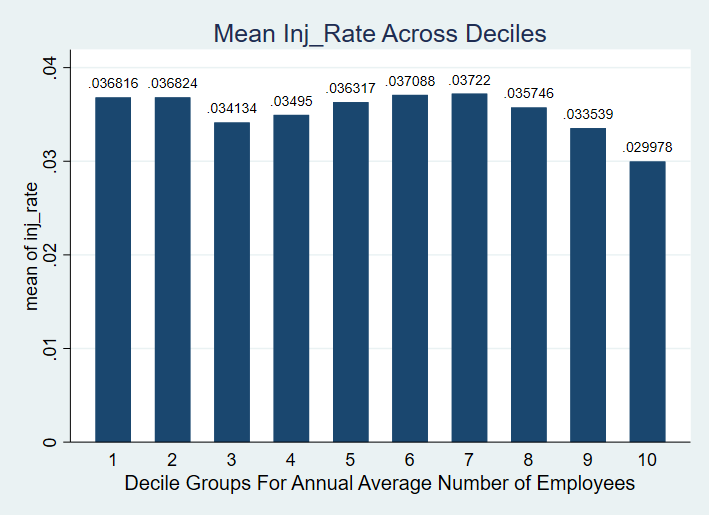
\includegraphics[width=0.7\linewidth]{Inj_RateDecileBar (3).png}
    \caption{Mean Injury Rate and Establishment Size}
    \label{Figure 1:}
\end{figure}

For the second part of our analysis, we aimed to break down the data into injury types. The reasoning for this is because the variable total injuries encapsulates several different injury types, all with different relationships with the decile variable. To provide more insight on this notion we have included three new variables, Total Poisonings Rate, Total Skin Disorders rate, and Total Respiratory Conditions rate. First, we examine how the poisoning rate varies across the establishment size distribution in Figure 2. From a first glance the first decile group has a much higher poisonings rate compared to the other nine. To explore this outlier, we first looked at summary statistics and found that the mean poisoning rate was .0000231 and the standard deviation was .0021069, and the median was 0. We chose to look through the data for possible outliers causing the smallest decile group to have the highest rate. We found that one observation had a Skin Disorder rate of exactly 1, implying that every person at that establishment had a skin disorder. Finally, we ran a correlation test and found a correlation coefficient of -.0025 which does not support our hypothesis because it highlights a subtle negative correlation between the two variables.

\begin{figure}
    \centering
    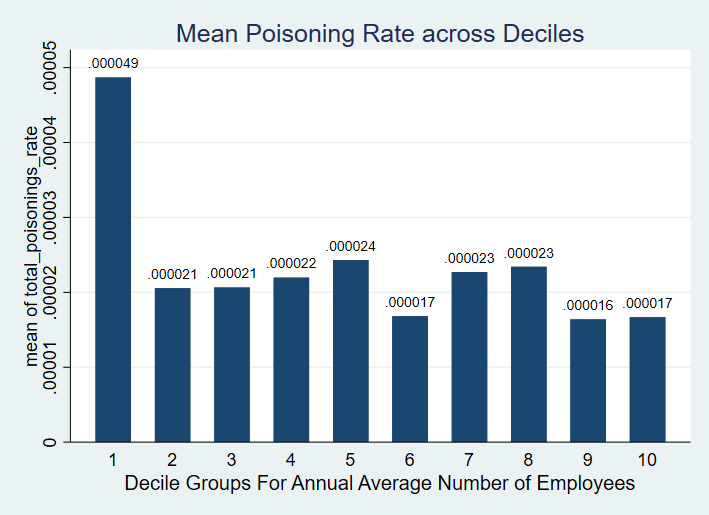
\includegraphics[width=0.7\linewidth]{PoisoningsDecileBar (2).png}
    \caption{The Distribution of The Total Poisoning Rate and Establishment Size}
    \label{Figure 2:}
\end{figure}


The next variable we looked at was the total skin disorders rate. As shown in Figure 3, we created a bar chart to analyze the relationship between the skin disorders rate and establishment size. At first glance it is hard to see if there is a correlation between the two variables, so we ran a correlation test and found a correlation coefficient of .0031. A correlation coefficient of 0.0031 suggests no correlation between the two variables. Additionally, the strength and direction of the relationship can vary based on the context of the data. We chose to look further into this relationship by looking at the mean skin disorder rate of .0001993, a range of 0 to 1, the standard deviation is .04745, and a median of 0. Compared to the main injury rate and the other types of injuries within our data this variable has a much smaller distribution with no huge outliers. The median of 0 also implies this injury does not occur much across establishments. 

\begin{figure}
    \centering
    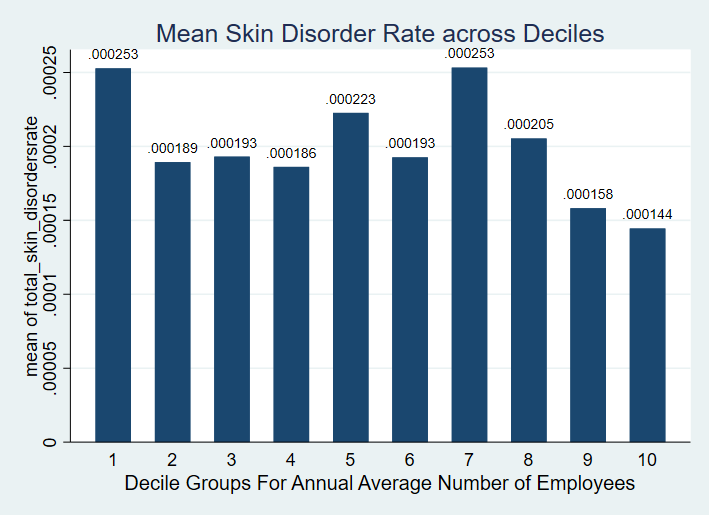
\includegraphics[width=0.7\linewidth]{SkinDecileBar (1).png}
    \caption{Mean Skin Disorder Rate and Establishment Size}
    \label{Figure 3:}
\end{figure}

The last injury rate we examine is for respiratory conditions. This variable measures the rate of respiratory issues reported within a year over the number of employees at a given firm. Figure 4 shows the relationship between firm size and the rate of respiratory conditions. The decile group with the highest respiratory rate was decile 8 which leads to questions about why? Is the correlation of this injury type sector based? To finalize our analysis, we ran a summary command and found a slightly large distribution with a range from 0 to 4.625.Implying that this variable may have more outliers than skin disorder injuries. We also found a mean of .00633, a standard deviation is .04745, and the median is 0. This shows that many of the establishments avoided respiratory issues but certain establishments must have been more prone than others with the range spanning so wide. 

\begin{figure}
    \centering
    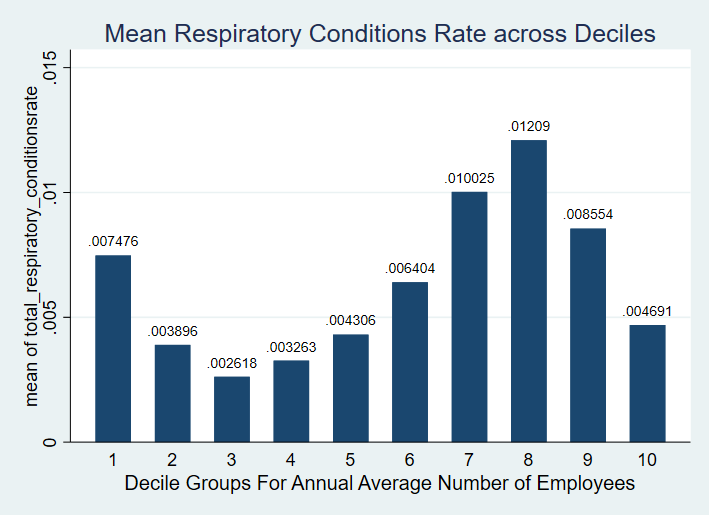
\includegraphics[width=0.7\linewidth]{RespiratoryDecileBar (1).png}
    \caption{Mean Respiratory Rate and Establishment Size}
    \label{Figure 4:}
\end{figure}

Finally, we wanted to include more about the variance of our data and provide further insight on the issues this data had with outliers. In doing so we created box plot to examine the different establishment size's injury rates to see if there were any trends in variance that were worth noting. The main takeaway from  this graph was that some establishment sizes had more outliers than others. For example, decile 1 had one observation in with an injury rate of 28. Decile 1 is the establishments with eight to nineteen people, meaning that some of these firms were having all eight employees injured 28 times. We also noticed that there was no trend in variance based on establishment size. This was not shocking based on the amount of outliers across the board but did highlight issues with data collection across all establishment sizes. This was also explored through the inclusion of median and mean comparison in our summary statistics because it highlights skewed distribution in the data and the large variance across all establishment sizes. 

\begin{figure}
    \centering
    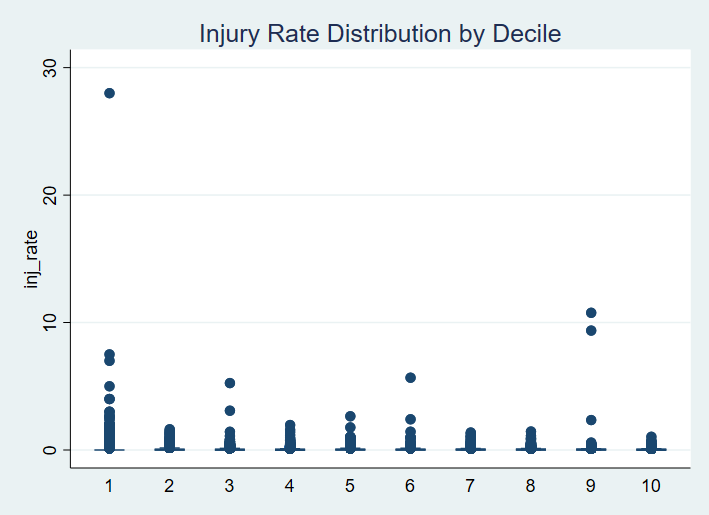
\includegraphics[width=0.8\linewidth]{InjRateBox.png}
    \caption{Injury Rate Distribution By Firm Size}
    \label{fig:enter-label}
\end{figure}

The core finding of our analysis highlights the amount extreme outliers and a limited correlation between injury rates and establishment size within the data set. While our initial hypothesis lacks robust support from this data, it serves as a catalyst for refining our approach in future studies on workplace safety. Despite the current data set's limitations, it lays the groundwork for future inquiries, offering valuable insights into potential hypotheses and nuances specific to distinct lines of work.  



\section{Discussion}
\label{sec:discussion}

 The data analysis and results above display potential issues with outliers and broken data within the data set. The data collected by OSHA is all establishment self-reports. Meaning that the number of accidents from individual establishments can be adjusted with little examination. The different policies that each establishment has for reporting and defining an accident may lead to the outliers within our results. For example, for an establishment with 3 employees it is highly unlikely that each employee would be injured 28 times, however, this was the case for one of our observations. For our research, there was no obvious way to avoid these extreme cases without unknowingly removing real data points. To continue this important research, it would be helpful to use another data set that had similar variables to compare the results to this data set. It would also be helpful for OSHA to adjust the way they collect data or at least increase the monitoring of data collection. In addition, it would be captivating to further study the variable of total respiratory conditions. Our results provided insight on how respiratory issue rates increase in certain decile groups, which may be due to the industry or could possibly point to an impact of COVID-19. We are curious about how reporting COVID-19 cases within the workplace has changed the data and how it contributes to the concept of work place accidents. In future studies, a deeper exploration of the total respiratory conditions in the year cases of 2019, 2020, 2021, and 2022 would be a necessary inclusion to understand the influence of COVID-19 on this variable. 


\section{Conclusion}
\label{sec:conclusion}

In this study, we investigate the potential correlation between injury rates and establishment size, utilizing data obtained from OSHA. Our analysis involves computing total injury rates for each establishment, examining rates for specific injury types (such as total skin disorders, respiratory conditions, and poisoning), and comparing mean rates across ten decile groups. The findings reveal minimal to no correlation between injury rates and establishment size, contrary to our initial hypothesis that larger establishments would experience lower injury rates per worker compared to smaller ones. To enhance this conclusion, further exploration could involve analyzing data from different years or sources. Additionally, when assessing the impact of establishment size on workplace accident rates, it is crucial to consider uncontrollable factors like reporting policies. Further investigation into  accident rates, including policy development and industry compositions, could also provide valuable insights. Overall, Addressing potential outliers within the data emerges as the next logical step in advancing our understanding of workplace accidents.

\newpage
\section*{Bibliography}
\doublespacing
\setlength\bibsep{0pt}

\indent Smith, Robert Stewart. “The Impact of OSHA Inspections on Manufacturing Injury Rates.” The Journal of Human Resources, vol. 14, no. 2, 1979, pp. 145–70. JSTOR, https://doi.org/10.2307/145640. Accessed 19 Dec. 2023. 

\indent Levine, David I et al. “Randomized government safety inspections reduce worker injuries with no detectable job loss.” Science (New York, N.Y.) vol. 336,6083 (2012)

\indent Viscusi, W. Kip. “The Impact of Occupational Safety and Health Regulation.” The Bell Journal of Economics, vol. 10, no. 1, 1979, pp. 117–40. JSTOR, https://doi.org/10.2307/3003322. Accessed 19 Dec. 2023. 

\indent Johnson, Charles K.K. M.S., S. J. “Demand conditions and worker safety: Evidence from Price shocks in mining”. National Bureau of economics reserch. 2019. Accessed 19 Dec. 2023.  

\indent Keiner, T. J., and Leeth, J. "Regulating Occupational and Product Risks." Handbook of the Economics of Risk and Uncertainty, edited by [Editor's Name], vol. [Volume Number], Publisher, Year, pp. 493-600. 

\indent Li, L., \& [Author's Middle Initial]. "The Effect of Workplace Inspections on Worker Safety." Sage, 2019, pp. 718-748. 

\indent Li, L. R. "The Effect of Labor Unions on Workplace." A Journal of Economy and Society, 2020, pp. 643-670. 

\indent United States. Occupational Safety and Health Administration. Occupational Safety and Health Administration, U.S. Department of Labor, 2023, [https://www.osha.gov/Establishment-Specific-Injury-and-Illness-Data]. 

\newpage
\section*{ Data Appendix} \label{sec:appendixa}
\addcontentsline{toc}{section}{Appendix A}

The data being used for this research project is from the Occupational Safety and Health Administration (OSHA). OSHA, the Occupational Safety and Health Administration, collects data primarily from private sector employers, including those in construction, general industry, and maritime. The agency's coverage extends to federal government employees, excluding those in the United States Postal Service. OSHA's data collection focuses on workplace injuries and illnesses, aiding in the enforcement of safety regulations and the identification of areas for improvement in various industries. We are using the most recent data set entitled "Establishment Specific Injury and Illness Data (Injury Tracking Application) CY2022"

\section*{Accessing OSHA Data Directions:}

\begin{enumerate}
  \item Go to the accidents team public repo by following this link: https://github.com/ecn310/course-project-accidentsteam
  \item Select the Reproducibility Folder 
  \item Press on the Data Folder 
  \item Inside the Data folder, press on the file entitled “ITA-data-cy2023.2 (1).zip”
  \item Press the Download button to download the zip file. This will download a CSV file of the data.
\end{enumerate}

\section*{Converting the CSV file to DTA Directions:}

\begin{enumerate}
  \item Find the CSV file in your downloads.
  \item Select "Extract All..." from the context menu.
  \item Choose the destination folder where you want to extract the contents.
  \item Import the CSV file into stata using the following code: import delimited "C:YOURPATH/ITA Data CY 2022 submitted thru 7-31-2023.csv", encoding(UTF-8). Make sure you change the path to where you downloaded the file!
  \item Then, use the following code to save the file as a STATA.dta file: save "Data.dta" you can change the location of where the file was saved using the "change directory" or "cd" command. NOTE: You do not need to use the replace command because it is good practice to keep the original data source.
\end{enumerate}

\section*{Opening Master Do-File}

\begin{enumerate}
  \item Go to accidents team repo page linked here: 
  https://github.com/ecn310/course-project-accidentsteam
  \item Open Reproduciblity Folder
  \item Download Master Do File 
  \item Make sure Stata is downloaded onto your desktop
  \item Open Master Do File, which will open Stata
  \item Change Directory using the CD command on line 65, this will put all of the graphs from the output into your selected folder. 
  \item Run the Master Do-file, any questions should be answered within in the notes on the file. 
  
\end{enumerate}



\end{document}